\documentclass[11pt]{article}
\usepackage{times}
\pagestyle{empty}
\parindent 0px
\usepackage{geometry}
 \geometry{
 a4paper,
 total={170mm,257mm},
 left=20mm,
 top=20mm,
 }
 
\title{CS5691: Assignment 2}
\author{Akshat Meena (CS19B052) \\ Rohit Bhagat (CS19B038)}
\date{}
\usepackage{graphicx}
\graphicspath{ {../Plots/} }

\begin{document}
\maketitle

\begin{center}
\begin{Large}
B. Bayesian Classifier
\end{Large}
\end{center}

\begin{enumerate}
	\begin{large}
	\item \textbf{Linearly Separable Data}
	\end{large}
	
	\begin{itemize}
		\item We observe that classification of linearly separable data can be done very easily. We get 100\% accuracy.
		\begin{figure}[h]
	\caption{
	\begin{small}
	Plot of PDF for case 1, 2, 3 respectively
	\end{small}
	}
	\centering
	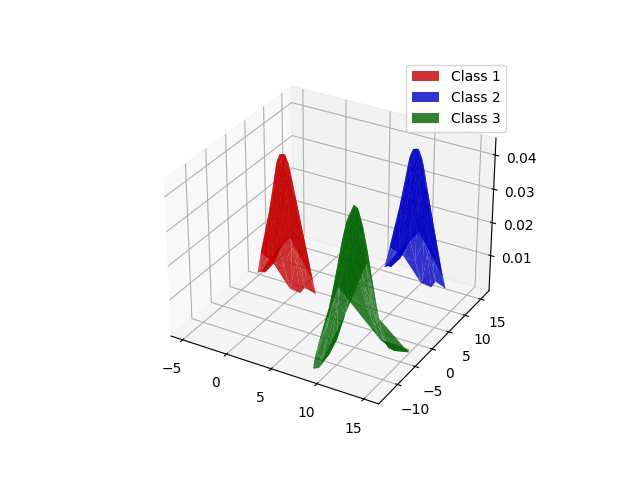
\includegraphics[scale=0.3]{LS_1}
	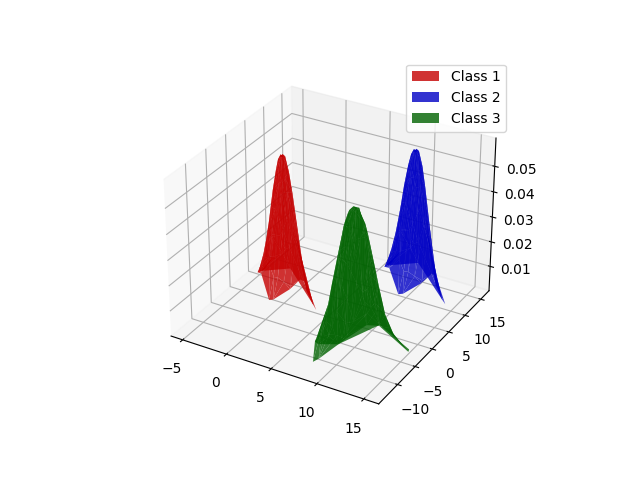
\includegraphics[scale=0.3]{LS_2}
	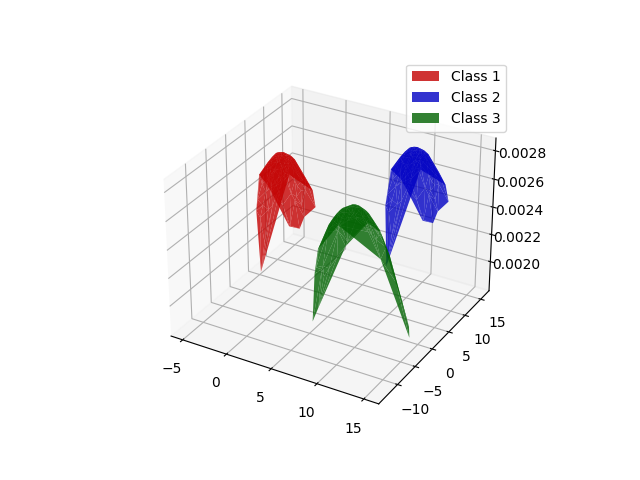
\includegraphics[scale=0.3]{LS_3}
	\end{figure}
	\end{itemize}
	
	\begin{large}
	\item \textbf{Non-Linearly Separable Data}
	\end{large}
	
	\begin{itemize}
		\item Below is the Gaussian PDF plot for Non-Linearly separable data for different cases
		\begin{figure}[h]
	\caption{
	\begin{small}
	Plot of PDF for case 1, 2, 3 respectively
	\end{small}
	}
	\centering
	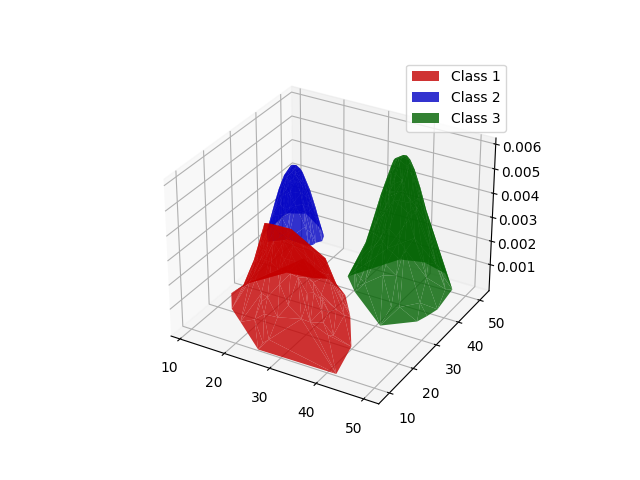
\includegraphics[scale=0.3]{NLS_1}
	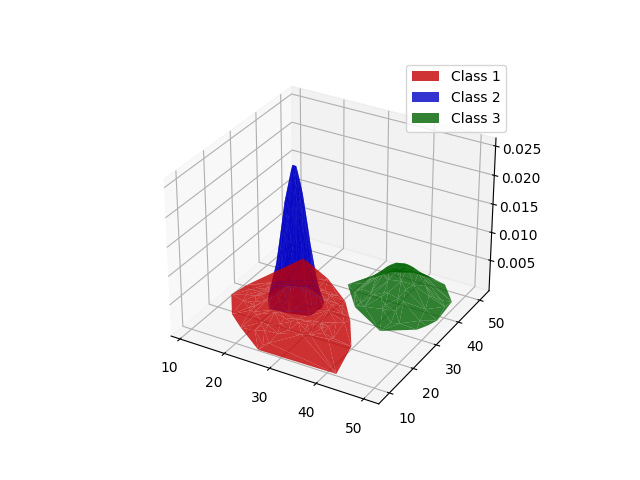
\includegraphics[scale=0.3]{NLS_2}
	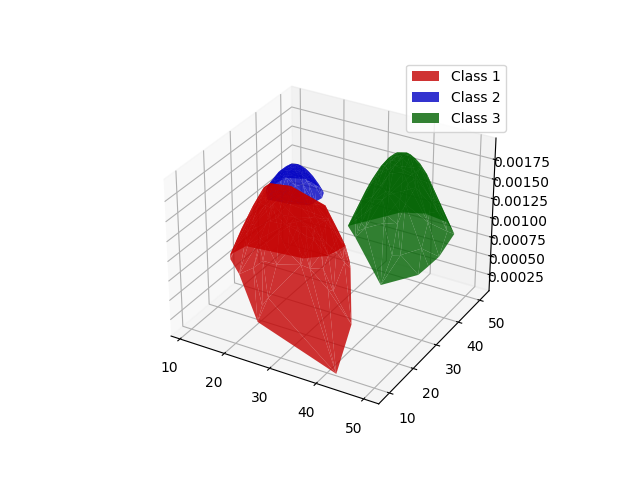
\includegraphics[scale=0.3]{NLS_3}
	\end{figure}
	\item DET curve for Non-Linearly seperable data
	\begin{figure}[h]
	\caption{
	\begin{small}
	DET Plot
	\end{small}
	}
	\centering
	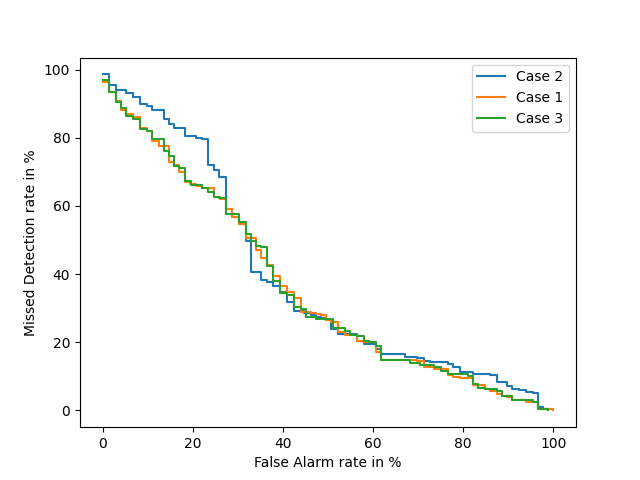
\includegraphics[scale=0.3]{NLS_DET}
	\end{figure}
	\end{itemize}
	
	\begin{large}
	\item \textbf{Real Data}
	\end{large}
	
	\begin{itemize}
		\item Below is the Gaussian PDF plot for Real data for different cases
		\begin{figure}[h]
	\caption{
	\begin{small}
	Plot of PDF for case 1, 2, 3 respectively
	\end{small}
	}
	\centering
	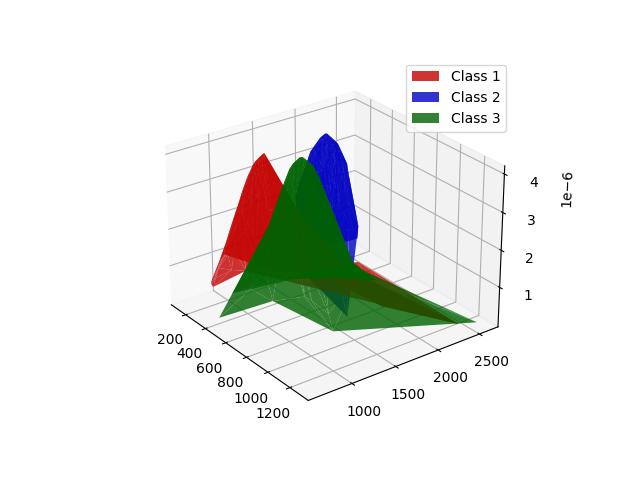
\includegraphics[scale=0.3]{RD_1}
	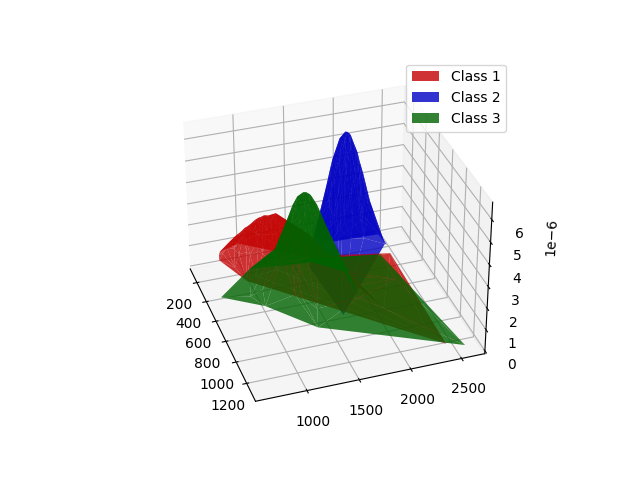
\includegraphics[scale=0.3]{RD_2}
	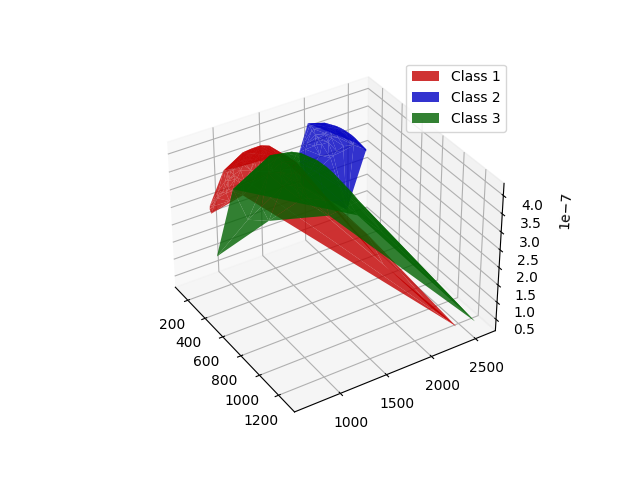
\includegraphics[scale=0.3]{RD_3}
	\end{figure}
	\item DET curve for Real data
	\begin{figure}[h]
	\caption{
	\begin{small}
	DET Plot
	\end{small}
	}
	\centering
	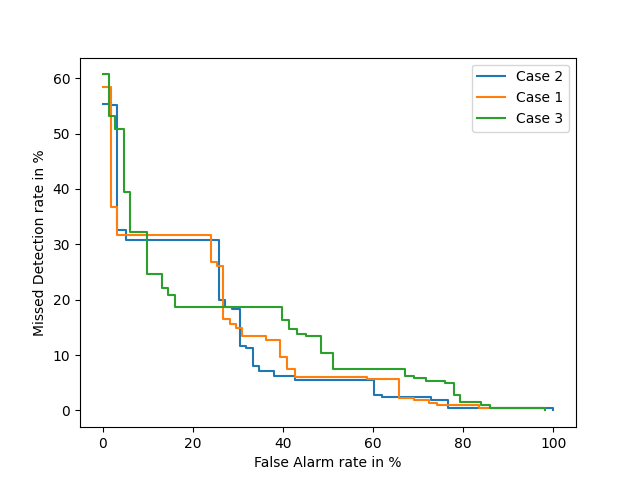
\includegraphics[scale=0.3]{RD_DET}
	\end{figure}
	\item Confusion Matrix for Real data
	\begin{figure}[h]
	\caption{
	\begin{small}
	Confusion Matrix
	\end{small}
	}
	\centering
	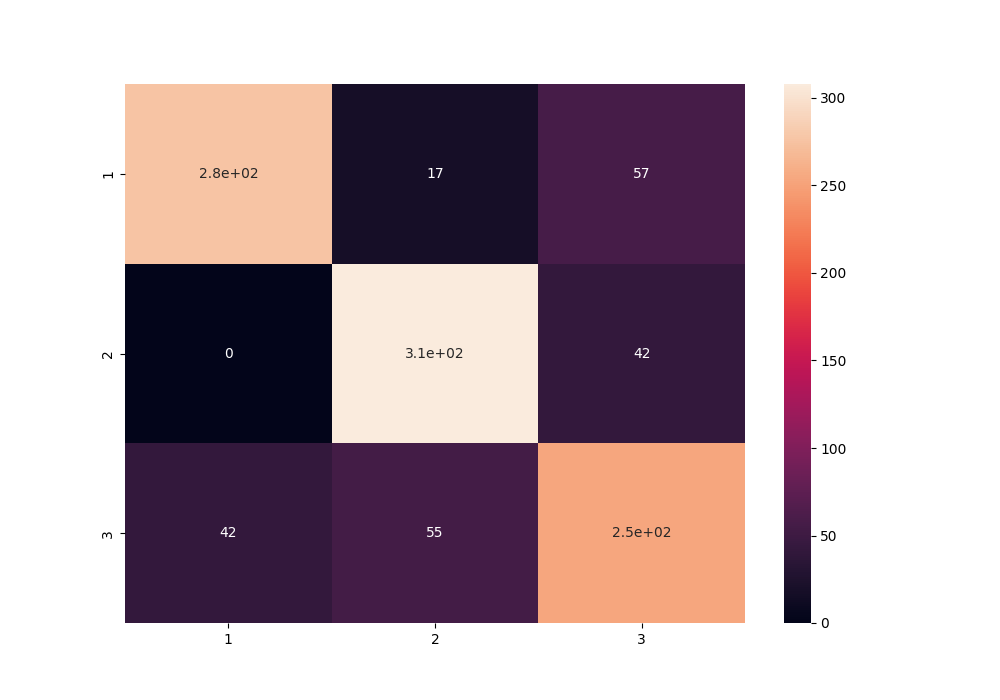
\includegraphics[scale=0.3]{RD_CM}
	\end{figure}
	\end{itemize}
	
\end{enumerate}

\end{document}